\begin{thms}
	Die Regelungstechnik (RT) besch�ftigt sich mit der selbstt�tigen gezielten Beeinflussung des
	Verhaltens von dynamischen Systemen.
\end{thms}

\begin{center}
	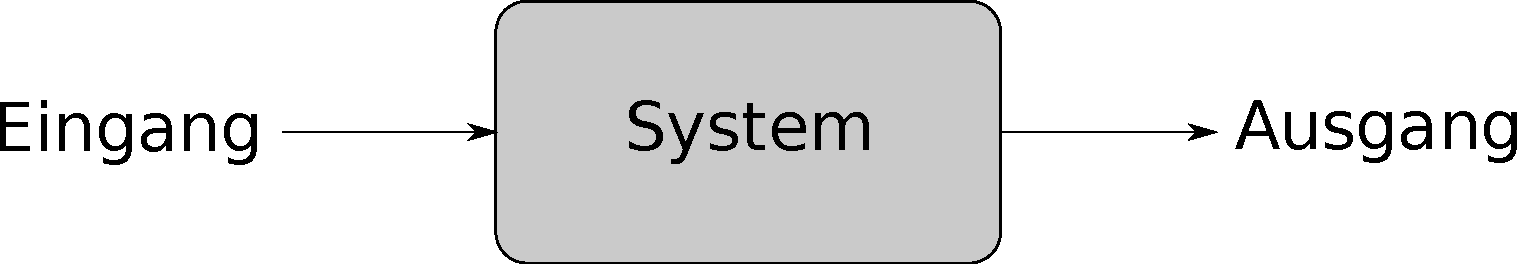
\includegraphics[width=300px]{graphics/system1.pdf}
\end{center}

Die Eing�nge werden in der RT aufgeteilt in von au�en vorgebbare \underline{Eingangsgr��en} und in durch die Umgebung festgelegte, st�rend wirkende \underline{St�rgr��en}. Von den Ausg�ngen werden nur diejenigen betrachtet, deren Verhalten unmittelbar interessiert. \underline{Ausgangsgr��en}.

\begin{center}
	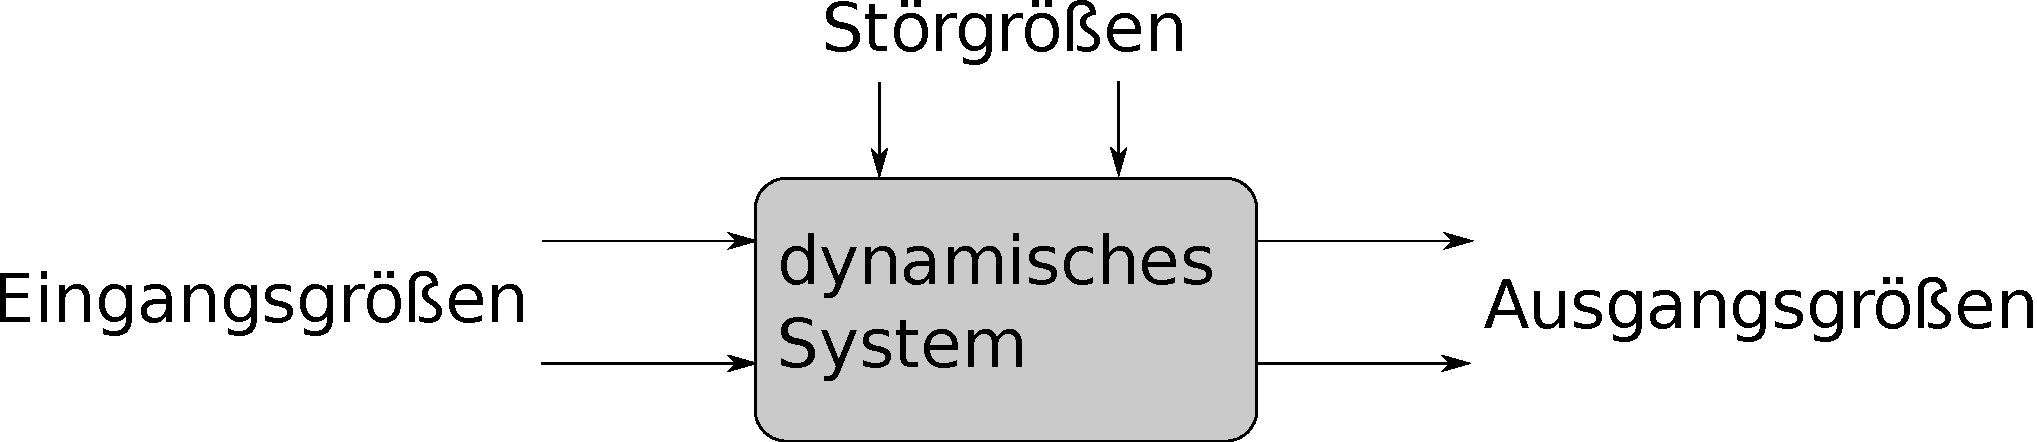
\includegraphics[width=300px]{graphics/dynsystem1.pdf}
\end{center}

\underline{Gezielte Beeinflussung} hei�t: Durch Vorgabe der Eingangsgr��enverl�ufe soll erreicht werden, dass die Ausgangsgr��en trotz St�reinwirkung ein gew�nschtes \underline{Sollverhalten} aufweisen.

\subsubsection*{Beispiel 1 (Raumtemperatur)}
\begin{center}
	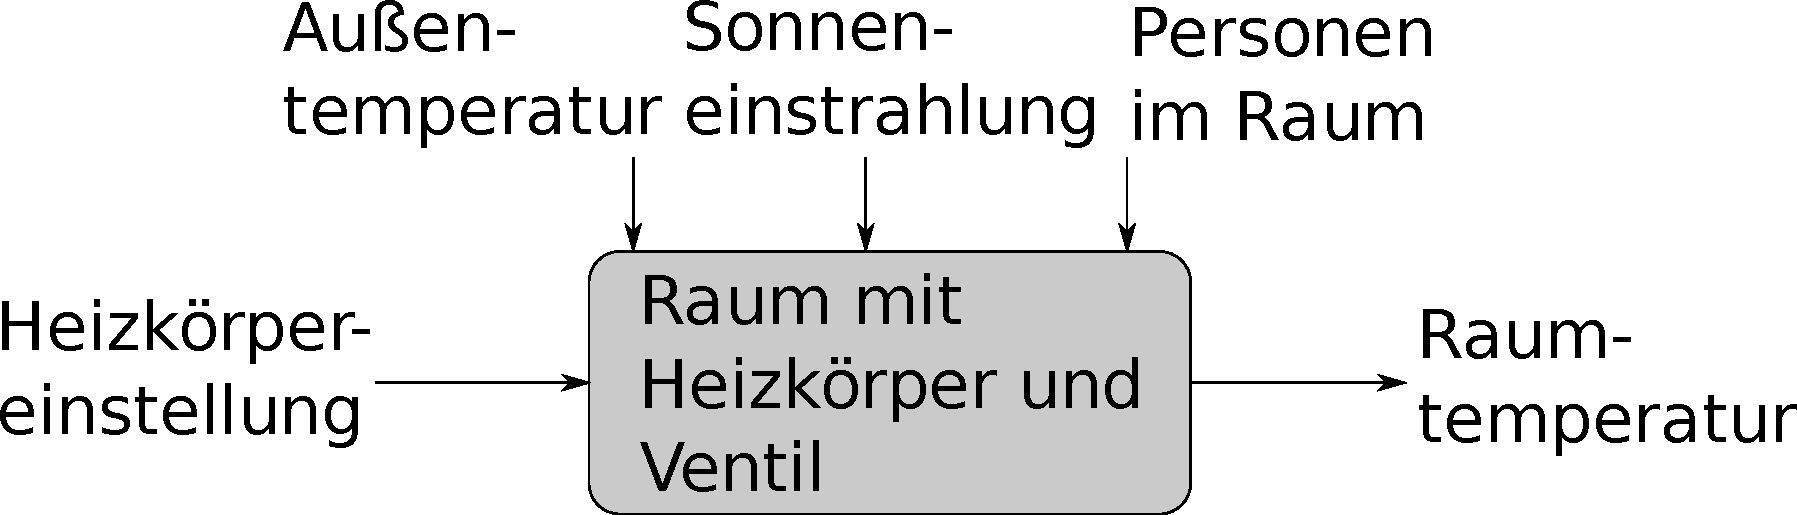
\includegraphics[width=300px]{graphics/raumtemperatur.pdf}
\end{center}

\subsubsection*{Beispiel 2 (Personenaufzug)}
\begin{center}
	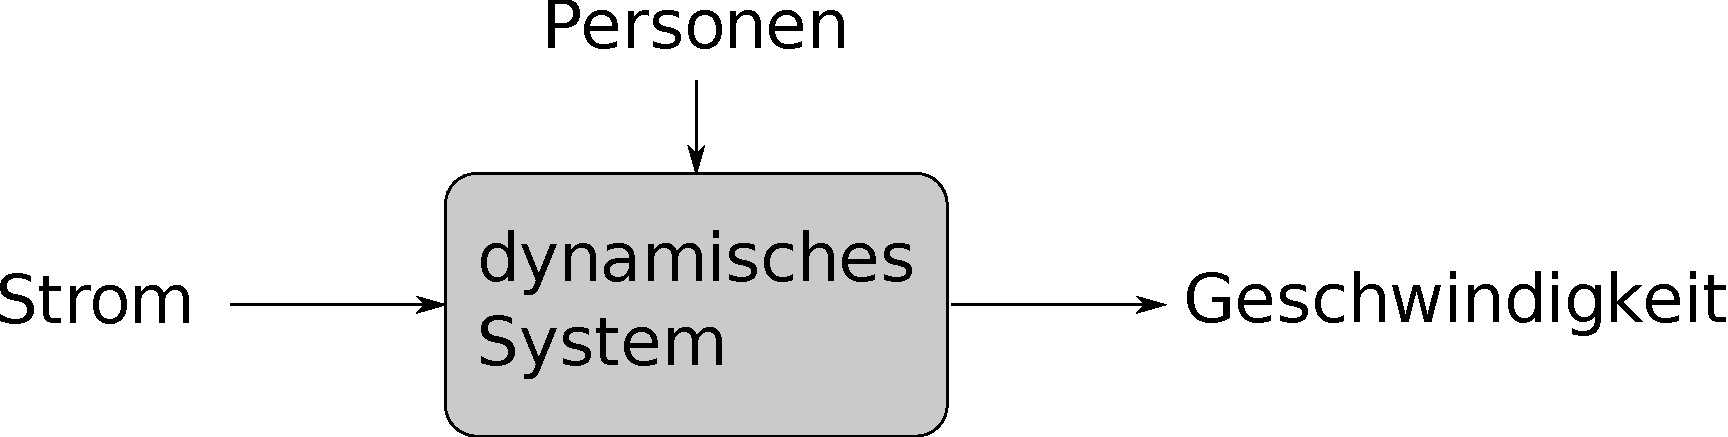
\includegraphics[width=300px]{graphics/personenaufzug.pdf}
\end{center}

\subsubsection*{Beispiel 3 (Auto fahren)}
\begin{center}
	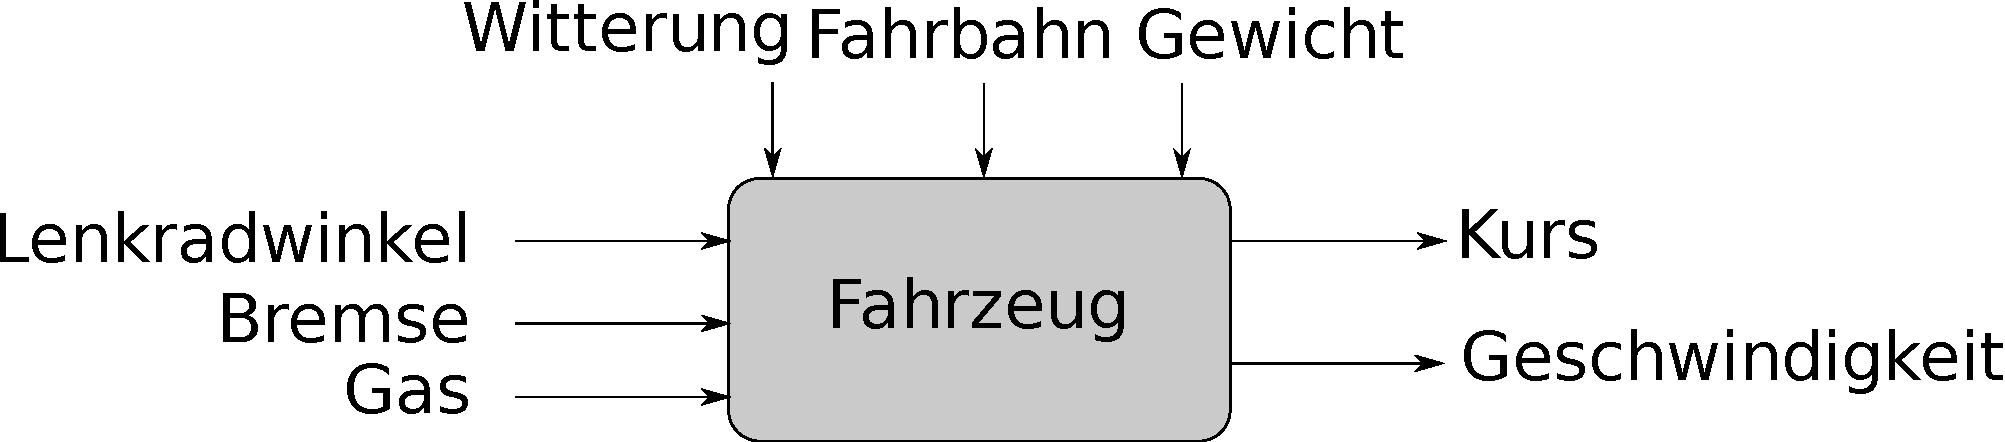
\includegraphics[width=300px]{graphics/autofahren.pdf}
\end{center}

\section*{Allgemeine Aufgabenstellung der RT}
Entwurf und Bereitstellung einer Einrichtung, die - hinzugef�gt zur Strecke - die Eingangsgr��en automatisch im gew�nschten Sinne generiert. \underline{Selbstt�tige gezielte Beeinflussung}.

\section*{Generelle Vorgehensweise zur L�sung}
\begin{enumerate}
	\item{mathematische Modellbildung der Strecke zur Abstraktion von deren physikalischen Auspr�gung und Erm�glichung der Anwendung universell einsetzbarer, systemtheoretisch fundierter Vorgehensweisen in Schritt 2. und 3.}
	\item{Analyse des Streckenverhaltens}
	\item{Entwurf der Steuer- und Regeleinrichtung}
	\item{Realisierung der Steuer- und Regeleinrichtung}
	\item{Inbetriebnahme und Erprobung des Gesamtsystems}
\end{enumerate}
